%%%%%%%%%%%%%%%%%%%%%%%%%%ch4-1
\begin{frame}[shrink]
  \frametitle{ch4.信号波形的检测}
  \framesubtitle{ch4-1. 统计检测理论基本概念及贝叶斯准则}
  \tableofcontents[hideallsubsections]
\end{frame}

\section{信号波形检测基本概念}

\begin{frame}{信号波形的检测基本内容}
\begin{itemize}
	\setlength{\itemsep}{.5cm}
	\item 掌握随机过程正交级数展开的目的和方法;
	\item 掌握高斯白噪声中二元确知信号波形的检测;
	\item 了解M元确知信号波形的检测;
	\item 将第三章有关统计检测的理论,推广至噪声中信号波形的最佳检测问题;
	\item 基本任务:根据性能要求,设计与环境相匹配的接收机;
	\item 主要问题:最佳检测的判决表达式,检测性能分析以及最佳波形设计等。	
\end{itemize}
\end{frame}

\begin{frame}{二元数字通信系统波形检测模型}
\centering
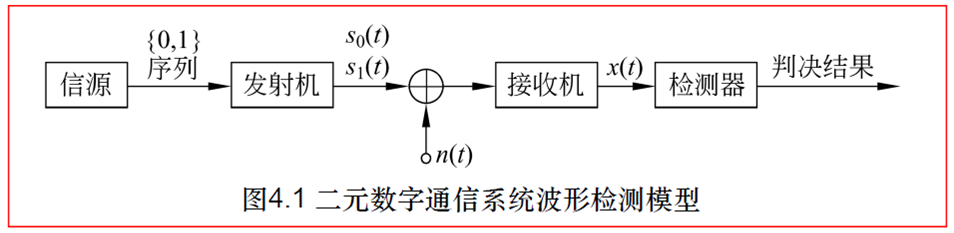
\includegraphics[scale=0.4]{4-1}\\
\begin{tabular}{cc}
	\textbf{信源输出} &\textbf{发射信号} \\ 
	0 & $s_0(t), nT\le t\le (n+1)T$ \\
	1 & $s_1(t), nT\le t\le (n+1)T$
\end{tabular} \\
~\\
\textbf{\textcolor{blue}{信号在信道传输中受到加性干扰}}
\begin{align*}
H_0: \quad x(t)=s_0(t)+n(t), \quad nT+t_0\le t\le (n+1)T+t_0\\
H_1: \quad x(t)=s_1(t)+n(t), \quad nT+t_0\le t\le (n+1)T+t_0
\end{align*}
\end{frame}

\begin{frame}{问题的提出}
\begin{itemize}
\item 第3章,统计检测理论处理的观测信号是$N$维矢量
\item 第4章,波形信号检测处理的是随机过程$x(t)$\\
\textcolor{red}{如何在两者之间建立联系?}\\
\textcolor{red}{能否利用第三章的方法,解决波形信号检测的问题?}
\end{itemize}
\pause
\textbf{\textcolor{blue}{比较上述两种不同的信号发现,如果能用一组随机变量来表示随机过程$x(t)$,  或者说将随机过程$x(t)$与一组随机变量之间建立联系,则可直接应用第三章的结果解决波形信号检测的问题。}}
\pause
\begin{itemize}
\item \textcolor{red}{如何用一组随机变量来表示一个随机过程?}
\end{itemize}
\pause
\textbf{\textcolor{blue}{信号由正交级数展开,可用展开系数和正交集来表示该信号。}}
\end{frame}

\section{随机过程的正交级数展开}

\begin{frame}{随机过程的正交级数展开}
\textbf{基本要求}\\
~\\
\begin{itemize}
	\setlength{\itemsep}{.5cm}
	\item 掌握随机过程的卡亨南---洛维展开
	\item 理解白噪声条件下, 正交函数集的任意性
	\item 理解参量信号随机过程的正交级数展开
\end{itemize}
\end{frame}

\section{信号分解为正交函数}

\begin{frame}{矢量正交与正交矢量集}
\begin{block}{矢量正交}
	$\bm{V_x}=(V_{x1},V_{x2},V_{x3})$与$\bm{V_y}=(V_{y1},V_{y2},V_{y3})$,正交的定义: 其\textbf{内积}为0。即
	\[\bm{V_xV_y}=\sum_{i=1}^{3}v_{xi}v_{yi}=0 \]
\end{block}
\begin{block}{正交矢量集}
	由两两正交的矢量组成的矢量集合称为\textbf{正交矢量集}。
\end{block}
\centering
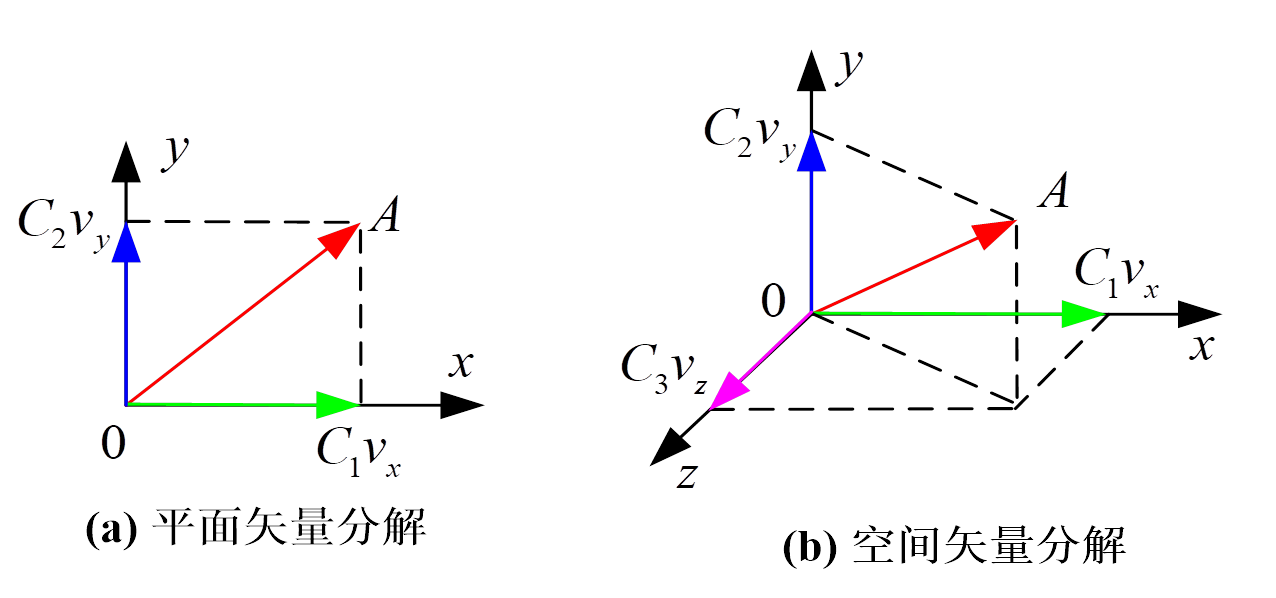
\includegraphics[scale=0.3]{vector}
\end{frame}

\begin{frame}
\begin{example}
如三维空间中,以矢量$\bm{v_x}=(2,0,0),\bm{v_y}=(0,2,0),\bm{v_z}=(0,0,2)$所组成的集合就是一个\textbf{正交矢量集}。\\
对于一个三维空间的矢量$\bm{A}=(2,5,8)$,可以用一个三维正交矢量集$\{\bm{v_x,v_y,v_z}\}$分量的线性组合表示。即
\[\bm{A=v_x+2.5v_y+4v_z} \]
\end{example}
\centering
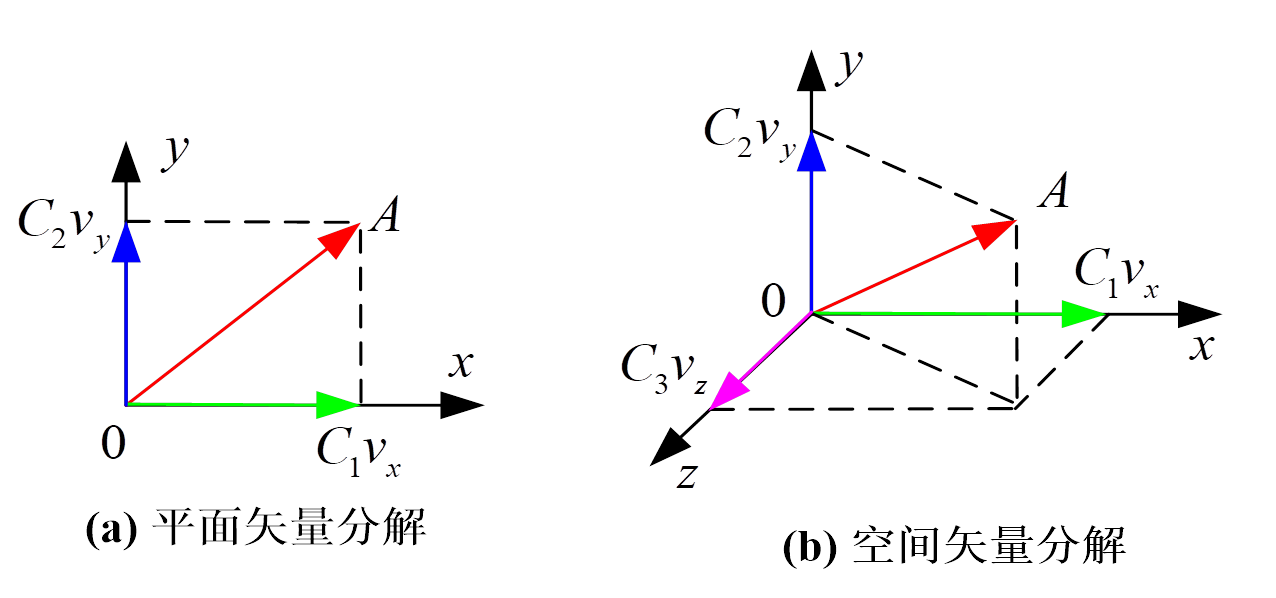
\includegraphics[scale=0.3]{vector}
\end{frame}

\begin{frame}{矢量空间正交分解的概念可推广到信号空间}
\begin{enumerate}
	\setlength{\itemsep}{.3cm}
	\item 在信号空间找到若干个\textbf{相互正交}的信号作为基本信号; 
	\item 使得信号空间中\textbf{任意信号均可表示成它们的线性组合}。
\end{enumerate}
\centering
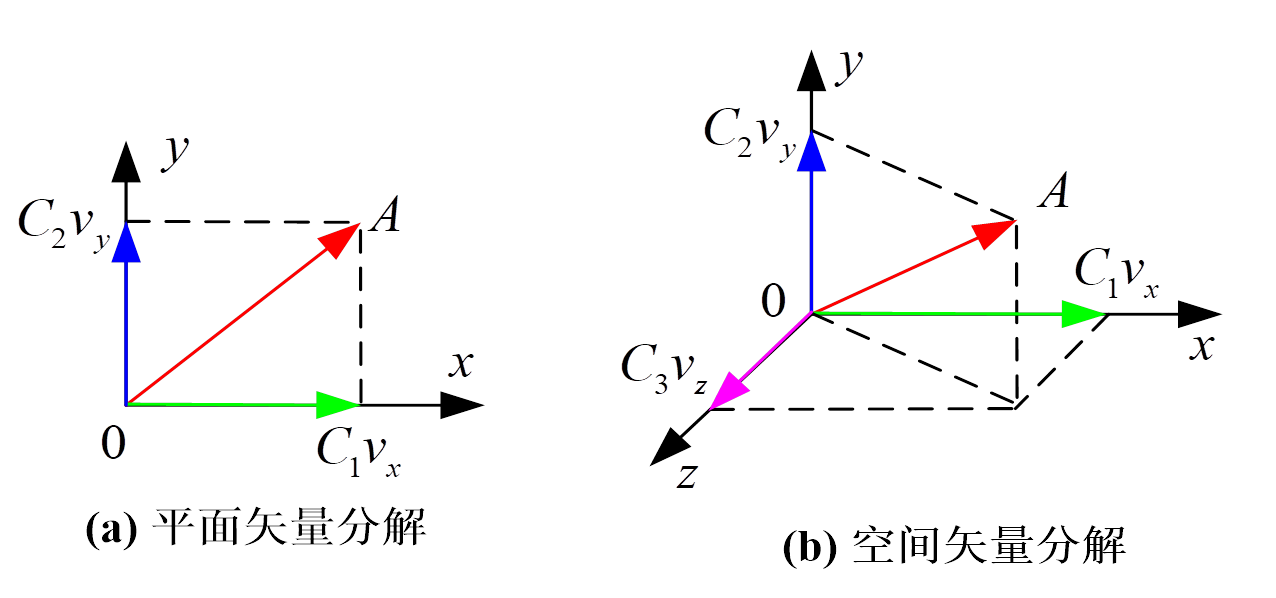
\includegraphics[scale=0.3]{vector}
\end{frame}

\begin{frame}{完备正交函数集}
三角函数集
\[ \{1,\cos(n\omega t),\sin(n\omega t),\dots\},n=1,2,\dots \]
就是在区间$(t_0,t_0,T),T=2\pi/\omega$上的\textbf{完备正交函数集}。
\begin{example}[傅里叶级数的三角形式]
\[ f(t)=\frac{a_0}{2}+\sum\limits_{n=1}^{\infty}a_n\cos(n\omega t)+\sum\limits_{n=1}^{\infty}b_n\sin(n\omega t)\]
傅里叶系数: 
\[ a_n=\frac{2}{T}\int_{-\frac{T}{2}}^{\frac{T}{2}}f(t)\cos(n\omega t)dt,\quad b_n=\frac{2}{T}\int_{-\frac{T}{2}}^{\frac{T}{2}}f(t)\sin(n\omega t)dt \]
\end{example}
\end{frame}

\begin{frame}{信号分解}
\begin{enumerate}
	\setlength{\itemsep}{.2cm}
	\item 在信号空间找到若干个\textbf{相互正交}的信号作为基本信号; 
	\item 使得信号空间中\textbf{任意信号均可表示成它们的线性组合}。
\end{enumerate}
\begin{columns}
	\column{0.4\textwidth}
	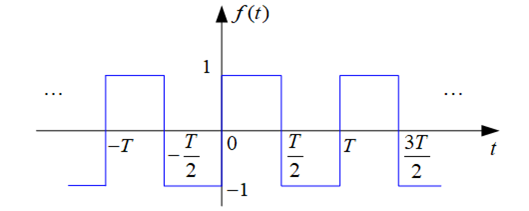
\includegraphics[scale=0.5]{4-2}
	\column{0.2\textwidth}
	\hspace{1cm}$\implies$
	\column{0.4\textwidth}
	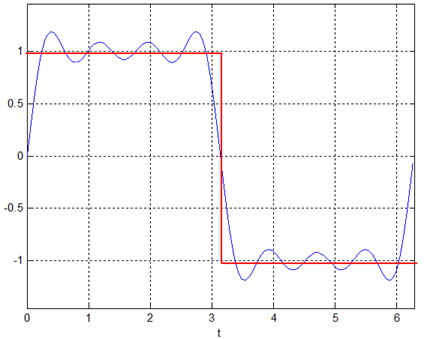
\includegraphics[scale=0.5]{4-3}
\end{columns}
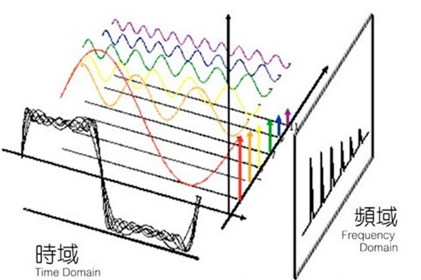
\includegraphics[scale=0.55]{4-4}
\end{frame}

\begin{frame}{正交级数展开}
\begin{table}[htbp!]
\small
%\centering
\caption{正交级数展开}
\begin{tabular}{|c|c|c|c|}
%\begin{tabular}{|p{1cm}|p{2cm}|p{2cm}|p{2cm}|}
\hline 
& 二维矢量 & 信号$f(t)$傅里叶展开 & 信号$x(t)$正交级数 \\ 
\hline 
\textbf{正交集} & $\{\bm{v_x,v_y}\}$ & $\{1,\cos(n\omega t),\sin(n\omega t)\}$ & $\{f_1(t),f_2(t),\dots,f_k(t)\}$ \\ 
\hline 
\textbf{展开系数} & $C_k=$矢量$\bm{A}$在 &
$a_n=\frac{2}{T}\int_{-\frac{T}{2}}^{\frac{T}{2}}f(t)\cos(n\omega t)dt$ & $x_k=\int_{0}^{T}x(t)f_k(t)dt$ \\  
(正交投影)& 第$k$个坐标的投影&$b_n=\frac{2}{T}\int_{-\frac{T}{2}}^{\frac{T}{2}}f(t)\sin(n\omega t)dt$& $$\\ 
\hline 
\textbf{线性表示} & $\bm{A}=C_1\bm{v_x}+C_2\bm{v_y}$ & $f(t)=\frac{a_0}{2}+\sum\limits_{n=1}^{\infty}a_n\cos(n\omega t)$ & $x(t)=\lim\limits_{N\to\infty}\sum\limits_{k=1}^{N}x_kf_k(t)$ \\ 
& & $+\sum\limits_{n=1}^{\infty}b_n\sin(n\omega t)$ &  \\ 
\hline 
\end{tabular} 
\end{table}
\end{frame}

\begin{frame}{完备正交函数集}
若实函数集$\{f_k(t)\} (k=1,2,\cdots)$, 在$(0,T)$时间内满足
\[
\int_{0}^{T}f_k(t)f_j(t)dt=
\begin{cases}
1, &j=k\\
0, &j\ne k
\end{cases}
\]
不存在函数$g(t)$, 满足
\[\int_{0}^{T}f_k(t)g(t)dt=0, \quad k=1,2,\cdots \]
则称函数集$\{f_k(t)\} (k=1,2,\cdots)$, 是\textbf{\textcolor{blue}{完备正交函数集}}。\\
~\\
\pause
比照矢量正交的定义:
\[\bm{V_xV_y}=\sum_{i=1}^{3}v_{xi}v_{yi}=0 \]
\end{frame}

\begin{frame}{确知信号的正交级数展开}
$s(t)$是定义在$(0, T)$时间内的确知信号, 且信号能量有限, 即
\[E_s=\int_{0}^{T}s^2(t)dt<\infty \]
该信号可用正交级数展开表示为:
\[s(t)=\lim\limits_{N\to\infty}\sum_{k=1}^{N}s_kf_k(t) \]
其中, $f_k(t)$是正交函数集的第$k$个\textcolor{blue}{坐标函数}, $s_k$是信号$s_k(t)$在第$k$个坐标函数上的\textcolor{blue}{正交投影}, 成为信号$s(t)$的第$k$个\textcolor{blue}{展开系数}, 且
\[ s_k=\int_{0}^{T}s(t)f_k(t)dt,\quad k=1,2,\cdots \]
\textbf{\textcolor{blue}{确知信号的展开系数$s_k(k=1,2,\cdots)$是确定的量, 而不是随机变量。}}
\end{frame}

\begin{frame}[shrink]{随机过程的正交级数展开}
\[\text{假设接收为信号: } x(t)=s(t)+n(t)\]
其中$s(t)$是确知信号, $n(t)$是零均值的平稳随机过程, 则接收信号$x(t)$也是平稳随机过程。由于随机过程是由很多样本函数构成的集合, 而每个样本函数是时间的函数, 所以对给定的样本函数$x(t)$, 可以进行正交级数展开
\[x(t)=\lim\limits_{N\to\infty}\sum_{k=1}^{N}x_kf_k(t), \quad \text{而展开系数为: }x_k=\int_{0}^{T}x(t)f_k(t)dt,\quad k=1,2,\cdots \]
\textcolor{blue}{展开系数$x_k$为一组随机变量}, 在平均意义上随机过程$x(t)$展开的均方误差等于0,或者说$\lim\limits_{N\to\infty}\sum\limits_{k=1}^{N}x_kf_k(t)$均方收敛于$x(t)$, 即$x_k$满足
\[\lim\limits_{N\to\infty}E\left[\left(x(t)-\sum_{k=1}^{N}x_kf_k(t)\right)^2 \right]=0 \]
\end{frame}

\begin{frame}{随机过程的正交级数展开}
\begin{block}{Notes}
\begin{align*}
&\textbf{随机过程: } x(t)=\lim\limits_{N\to\infty}^N\sum\limits_{k=1}^Nx_kf_k(t)\\
&\textbf{展开系数: } x_k=\int_{0}^{T}x(t)f_k(t)dt,\quad k=1,2,\dots
\end{align*}
随机过程$x(t)$可以由上式求得的展开系数$x_k$来恢复,就是说$x(t)$完全由展开系数$x_k$确定。注意,这里对随机过程$x(t)$进行正交级数展开所用的正交函数集$\{f_k(t)\}$并没有提出特别的要求,所以\textbf{展开系数$x_k(k=1,2,\dots)$之间可能是相关的随机变量}。\\
\end{block}
\textbf{问题:} 如何根据噪声干扰的特性,正确选择随机过程展开的正交函数集$\{f_k(t)\}$,以使\textbf{展开系数$x_k$之间是互不相关的随机变量}。
\end{frame}

\section{随机过程的卡亨南---洛维展开}

\begin{frame}{随机过程的卡亨南---洛维展开: 预备公式}
\begin{itemize}
\item 随机过程: $x(t)=s(t)+n(t)$
\item $\{f_k(t)\}$是一组正交函数集, $k=1,2,\dots$
\item 随机过程$x(t)的$正交展开系数$x_k$是一个\textbf{随机变量}: $x_k=\int_{0}^{T}x(t)f_k(t)dt$
\item 确知信号$s(t)$正交展开系数$s_k$是一个\textbf{确定的量}: $s_k=\int_{0}^{T}s(t)f_k(t)dt$
\item 确知信号$s(t)$的展开系数$s_k$为确定的量,其均值就是本身: $E(s_k)=E\left[\int_{0}^{T}s(t)f_k(t)dt\right]=\int_{0}^{T}E[s(t)]f_k(t)dt=\int_{0}^{T}s(t)f_k(t)dt=s_k$
\item 噪声$n(t)$是一个\textbf{零均值}的平稳随机过程:
\begin{itemize}
\item[-] $E[n(t)]=0$
\item[-]  $n(t)$的自相关函数只取决于时间间隔$(t_k-t_j)$, 而与时间的起始时刻无关, $E[n(t_j)n(t_k)]=r_n(t_k-t_j)$
\end{itemize}
\end{itemize}
\end{frame}

\begin{frame}[shrink]{随机过程的卡亨南---洛维展开}
\textbf{\textcolor{blue}{目的:给出一种正交函数集的选择方法,以保证展开系数之间是互不相关的随机变量。}}
随机过程: $x(t)=s(t)+n(t)$, 正交函数集$\{f_k(t)\}$, $x(t)$的各展开系数$x_k$是随机变量, 当随机过程$x(t)$满足
\[\int_{0}^{T}x^2(t)dt<\infty \]
时, 其展开系数$x_k$的均值为
\begin{align*}
E[x_k]&=E\left[\int_{0}^{T}x(t)f_k(t)dt\right]=E\left[\int_{0}^{T}\left(s(t)+n(t)\right)f_k(t)dt\right]\\
&=E\left[\int_{0}^{T}s(t)f_k(t)dt+\int_{0}^{T}n(t)f_k(t)dt\right]=E\left[\int_{0}^{T}s(t)f_k(t)dt\right]+E\left[\int_{0}^{T}n(t)f_k(t)dt\right]\\
&=E\left[\int_{0}^{T}s(t)f_k(t)dt\right]+\int_{0}^{T}E[n(t)]f_k(t)dt \qquad  (\text{by }E[n(t)]=0)\\
&=E\left[\int_{0}^{T}s(t)f_k(t)dt\right]=E[s_k] = s_k\quad \text{(by 确知展开系数的均值就是本身)}
\end{align*}
\end{frame}

\begin{frame}[shrink]{随机过程的卡亨南---洛维展开}
展开系数$x_j$与$x_k$协方差是在t时刻两个随机变量减去各自的均值后的乘积。
\begin{align*}
&E[(x_j-E(x_j))(x_k-E(x_k))]=E[(x_j-s_j)(x_k-s_k)]\\
&=E\left[\left(\int_{0}^{T}x(t)f_j(t)dt-s_j\right)\left(\int_{0}^{T}x(t)f_k(t)dt-s_k\right)\right]\\
&=E\left[\left(\int_{0}^{T}(s(t)+n(t))f_j(t)dt-s_j\right)\left(\int_{0}^{T}(s(t)+n(t))f_k(t)dt-s_k\right)\right]\\
&=E\left[\left(\int_{0}^{T}n(t)f_j(t)dt\right)\left(\int_{0}^{T}n(t)f_k(t)dt\right)\right]=E\left[\left(\int_{0}^{T}n(t)f_j(t)dt\right)\left(\int_{0}^{T}n(u)f_k(u)du\right)\right]\\
&=E\left[\int_{0}^{T}f_j(t)\left[\int_{0}^{T}n(t)n(u)f_k(u)du\right]dt\right]=\int_{0}^{T}f_j(t)\left[\int_{0}^{T}E[n(t)n(u)]f_k(u)du\right]dt\\
&=\int_{0}^{T}f_j(t)\left[\int_{0}^{T}r_n(t-u)f_k(u)du\right]dt\quad (\text{by }E[n(t_j)n(t_k)]=r_n(t_k-t_j))
\end{align*}
\end{frame}

\begin{frame}{随机过程的卡亨南---洛维展开}
希望$x(t)$各展开系数$x_j$与$x_k$的协方差满足:
\[E[(x_j-E(x_j))(x_k-E(x_k))]=E[(x_j-s_j)(x_k-s_k)]=\lambda_k\delta_{jk} \]
式中$\delta_{jk}=
\begin{cases}
1, & (j=k)\\
0, & (j\ne k)
\end{cases}$, \quad $\lambda_k$是展开系数$x_k$的方差, $k=1,2,\dots$\\
~\\
这样,\\
当$j\ne k$时, $E[(x_j-s_j)(x_k-s_k)]=0$, 即展开式的各展开系数之间互不相关;\\ 当$j=k$时, $E[(x_j-s_j)(x_k-s_k)]=E[(x_j-s_k)^2]=\lambda_k$, 是展开系数$x_k$的方差。
\end{frame}

\begin{frame}{随机过程的卡亨南-洛维展开}
展开系数$x_j$与$x_k$协方差:
\[E[(x_j-s_j)(x_k-s_k)]=\int_{0}^{T}f_j(t)\left[\int_{0}^{T}r_n(t-u)f_k(u)du\right]dt \]
其中, $x(t)=s(t)+n(t)(0\le t\le T),r_n(t-u)=E[n(t)n(u)]$是零均值平稳噪声过程$n(t)$的自相关函数。

为保证$E[(x_j-s_j)(x_k-s_k)]=\lambda_k\delta_{jk}$
\[\int_{0}^{T}r_n(t-u)f_k(u)du=\lambda_kf_k(t), \quad 0\le t\le T \]
该式是齐次积分方程。该方程的解$f_k(t)$就是正交函数集$\{f_k(t) \}$的第$k$个坐标函数。
\[ E[(x_j-s_j)(x_k-s_k)]=\lambda_k\int_{0}^{T}f_j(t)f_k(t)dt=\lambda_k\delta_{jk} \implies f_j(t)\text{与}f_k(t)\text{正交。}\] 
\end{frame}

\section{白噪声条件下正交函数集的任意性}

\begin{frame}{白噪声条件下正交函数集的任意性(1)}
假设接收信号为$x(t)=s(t)+n(t)$, $n(t)$是零均值,功率谱密度为$P_n(\omega)=N_0/2$的白噪声,其自相关函数为: $r_n(t-u)=\frac{N_0}{2}\delta(t-u)$, (说明噪声自相关函数在$t=u$时不为0,其他时刻都为0,自相关性最强)\\
对于任意正交函数集$\{f_k(t)\}$,展开系数$x_j$与$x_k$协方差:
\begin{align*}
E[(x_j-s_j)(x_k-s_k)]&=\int_{0}^{T}f_j(t)\left[\int_{0}^{T}r_n(t-u)f_k(u)du\right]dt\\
&=\frac{N_0}{2}\int_{0}^{T}f_j(t)\left[\int_{0}^{T}\delta(t-u)f_k(u)du\right]dt\\
&=\frac{N_0}{2}\int_{0}^{T}f_j(t)f_k(t)dt=\frac{N_0}{2}\delta_{jk}
\end{align*}
式中$\delta_{jk}=
\begin{cases}
1, & (j=k)\\
0, & (j\ne k) 
\end{cases},\quad
\delta(t-u)=
\begin{cases}
1, & (t=u)\\
0, & (t\ne u) 
\end{cases}
$
\end{frame}

\begin{frame}{白噪声条件下正交函数集的任意性(2)}
假设接收信号为$x(t)=s(t)+n(t)$, $n(t)$是零均值,功率谱密度为$P_n(\omega)=N_0/2$的白噪声,其自相关函数为: 
\[r_n(t-u)=\frac{N_0}{2}\delta(t-u)\]
对于任意正交函数集$\{f_k(t)\}$,展开系数$x_j$与$x_k$协方差:
\begin{align*}
E[(x_j-s_j)(x_k-s_k)]=\int_{0}^{T}f_j(t)\left[\int_{0}^{T}r_n(t-u)f_k(u)du\right]dt=\frac{N_0}{2}\delta_{jk}
\end{align*}
\begin{block}{重要结论}
当$j\ne k$时,展开系数$x_j$与$x_k$协方差=0。这说明,在$n(t)$是白噪声的条件下,取任意正交函数集$\{f_k(t)\}$对平稳随机过程$x(t)$进行展开,其展开系数$x_k(k=1,2,\dots)$之间都是互不相关的。这就是\textbf{\textcolor{blue}{白噪声条件下正交函数集的任意性}}。
\end{block}
\end{frame}

\section{参量随机信号时随机过程的正交级数展开}

\begin{frame}[shrink]{参量随机信号时随机过程的正交级数展开}
接收信号为含有参量$\bm{\theta}$的平稳随机过程信号
\[x(t)=s(t; \bm{\theta})+n(t),\quad 0\le t\le T \]
把参量信号$s(t; \bm{\theta})$看作以$\bm{\theta}$为条件的信号, 正交函数集为$\{f_k(t)\}$, 则$x(t)$展开为
\[x(t)=\lim\limits_{N\to\infty}\sum_{k=1}^{N}x_kf_k(t) \]
展开系数为
\begin{align*}
x_k=\int_{0}^{T}x(t)f_k(t)dt=\int_{0}^{T}[s(t; \bm{\theta})+n(t)]f_k(t)dt=s_{k|\bm{\theta}}+n_k,\quad k=1,2,\cdots
\end{align*}
$s_{k|\bm{\theta}}$是信号$s(t; \bm{\theta})$以$\bm{\theta}$为条件的展开系数, 即
\[s_{k|\bm{\theta}}=\int_{0}^{T}s(t; \bm{\theta})f_k(t)dt,\quad  k=1,2,\cdots \]
\end{frame}

\begin{frame}[shrink]{参量随机信号时随机过程的正交级数展开}
$x(t)$展开系数的条件均值为
\begin{align*}
E[x_k]=E[s_{k|\bm{\theta}}+n_k]=E[s_{k|\bm{\theta}}]=s_{k|\bm{\theta}}
\end{align*}
为使展开系数互不相关,则
\[E[(x_j-s_{j|\bm{\theta}})(x_k-s_{k|\bm{\theta}})]=\lambda_k\delta_{jk} \]
若$n(t)$的自相关函数为$r_n(t-u)$时, $x_k$互不相关的正交函数集$\{f_k(t)\}$满足齐次方程
\[\int_{0}^{T}r_n(t-u)f_k(u)du=\lambda_kf_k(t), \quad 0\le t\le T \]
~\\
\textbf{\textcolor{blue}{在白噪声条件下,正交函数集仍具有任意性。}}
\end{frame}
